\section{Quadratura de Riemann}\label{quarie}

Em problemas multidimensionais, a densidade marginal correspondente a cada variável aleatória para a qual se deseja fazer inferência é obtida integrando a densidade conjunta sobre as demais. Frequentemente, o cálculo das integrais pode ser difícil ou mesmo impossível analiticamente. No caso de uma densidade \textit{a posteriori} conjunta deve-se aproximar algumas das, ou todas as, integrais associadas a cada densidade \textit{a posteriori} marginal de interesse por métodos numéricos, os quais podem ser determinísticos ou estocásticos. Neste presente trabalho, isto será feito para todos os 3 parâmetros do modelo de mistura finita de normais com variância contaminada.

Dentre os métodos determinísticos mais usuais, para a aproximação das integrais correspondentes às densidades \textit{a posteriori} marginais de $\mu$, $\sigma^2$ e $\nu$, será utilizado o método da quadratura de Riemann, um caso particular e o mais simples da família das \textit{fórmulas de Newton-Cotes} (Chapra, 2015)\cite{Chapra2015}, as quais substituem o verdadeiro integrando por uma aproximação polinomial dentro de cada subintervalo contido no intervalo de integração. Na quadratura de Riemann, o integrando avaliado em cada subintervalo é aproximado por uma função constante avaliada no limite inferior (ou superior) do mesmo subintervalo.

Aproximações polinomiais com nós igualmente espaçados a cada subintervalo, como as regras de quadratura do Trapézio (grau 1) ou de Simpson (grau 2), obtém resultados com menor erro do que a quadratura de Riemann. Quando o grau da aproximação polinomial tende ao infinito, a quadratura converge para o verdadeiro valor da integral. Porém, em problemas de dimensão igual a 2 ou superior, usar aproximações polinomiais com nós torna-se muito custoso computacionalmente, uma vez que temos três ou mais termos na soma que aproximará a integral para cada dimensão. Por esta razão, escolheu-se a quadratura de Riemann para obter densidades \textit{a posteriori} marginais de $\mu$, $\sigma^2$ e $\nu$, pois esta regra possui um único termo na soma aproximadora, facilitando a programação das rotinas iterativas associadas. Em uma dada aproximação, o mesmo número de intervalos será usado para todas as dimensões.

Antes de aproximar as densidades \textit{a posteriori} marginais de cada parâmetro, é necessário aproximar o inverso da constante de proporcionalidade. Dados três parâmetros $(\alpha_1, \alpha_2, \alpha_3)$ e uma amostra dos dados $\bm{y}$ quaisquer, suponha que se deseja aproximar a densidade \textit{a posteriori} marginal de $\alpha_3$ dados os pontos $r_i, s_j, t_k$ da grade formada por todos os subintervalos de integração, $i, j, k \in \{1, \ldots, L\}$. Temos pela quadratura de Riemann que
\begin{align}
p(\alpha_3 | \bm{y})
&= \iint p(\alpha_1, \alpha_2, \alpha_3 | \bm{y}) d\alpha_1 d\alpha_2 \nonumber \\
\Rightarrow p(t_k | \bm{y})
&= \iint p(\alpha_1, \alpha_2, t_k | \bm{y}) d\alpha_1 d\alpha_2 \approx \sum_{i=1}^{L} \sum_{j=1}^{L} p(r_i, s_j, t_k | \bm{y}) \Delta_i \Delta_j \nonumber \\
&= \sum_{i=1}^{L} \sum_{j=1}^{L} c \cdot h(r_i, s_j, t_k | \bm{y}) \Delta_i \Delta_j. \label{eq:dpm_riem}
\end{align}

Como $c$, a constante de proporcionalidade, é dada pelo inverso da densidade \textit{a priori} preditiva $f(\bm{y})$, a qual é obtida integrando-se em todo o espaço paramétrico o produto entre a função de verossimilhança $f(\bm{y} | \alpha_1, \alpha_2, \alpha_3)$ e as densidades (ou funções de probabilidade) \textit{a priori} para $\alpha_1$, $\alpha_2$ e $\alpha_3$, também é possível aproximar $c$ pela quadratura de Riemann. Neste caso, $c^{-1} \approx \sum_{i=1}^{L} \sum_{j=1}^{L} \sum_{k=1}^{L} h(r_i, s_j, t_k | \bm{y}) \Delta_i \Delta_j \Delta_k$. Com o valor aproximado para $c$, é possível calcular \eqref{eq:dpm_riem} nos limites superior e inferior de todos os subintervalos de um dado parâmetro e enfim obter uma aproximação da densidade \emph{a posteriori} marginal deste mesmo parâmetro através de uma curva gráfica que liga todos os valores calculados. Evidentemente, quanto menor o tamanho de cada subintervalo, melhor a curva traçada aproximará a verdadeira densidade.

Para o modelo de mistura finita de normais com variância contaminada foram consideradas três quantidades distintas de subintervalos, correspondentes aos 3 cenários para a aproximação via quadratura de Riemann: $L = \{15, 50, 100\}$. Em cada cenário, dividiram-se os três intervalos de massa probabilística obtidos nas Figuras \ref{fig:maspro_mu} a \ref{fig:maspro_nu} pelo respectivo valor de $L$. Nos três cenários, os valores calculados para o inverso da constante de proporcionalidade foram bem próximos: $3.9071 \times 10^{-229}$ para $L = 15$; $3.9014 \times 10^{-229}$ para $L = 50$ e $3.8999 \times 10^{-229}$ para $L = 100$. Com tais valores de $c^{-1}$, foram estimadas as densidades \textit{a posteriori} marginais para $\mu, \sigma^2$ e $\nu$, cujas curvas são apresentadas nas Figuras \ref{fig:dpm_mu_qr_15} a \ref{fig:dpm_nu_qr_15}; \ref{fig:dpm_mu_qr_50} a \ref{fig:dpm_nu_qr_50} e \ref{fig:dpm_mu_qr_100} a \ref{fig:dpm_nu_qr_100}:

\begin{figure}[t]%
	\centering
	\subfloat[Densidade \textit{a posteriori} de $\mu$]{{
			\label{fig:dpm_mu_qr_15}
			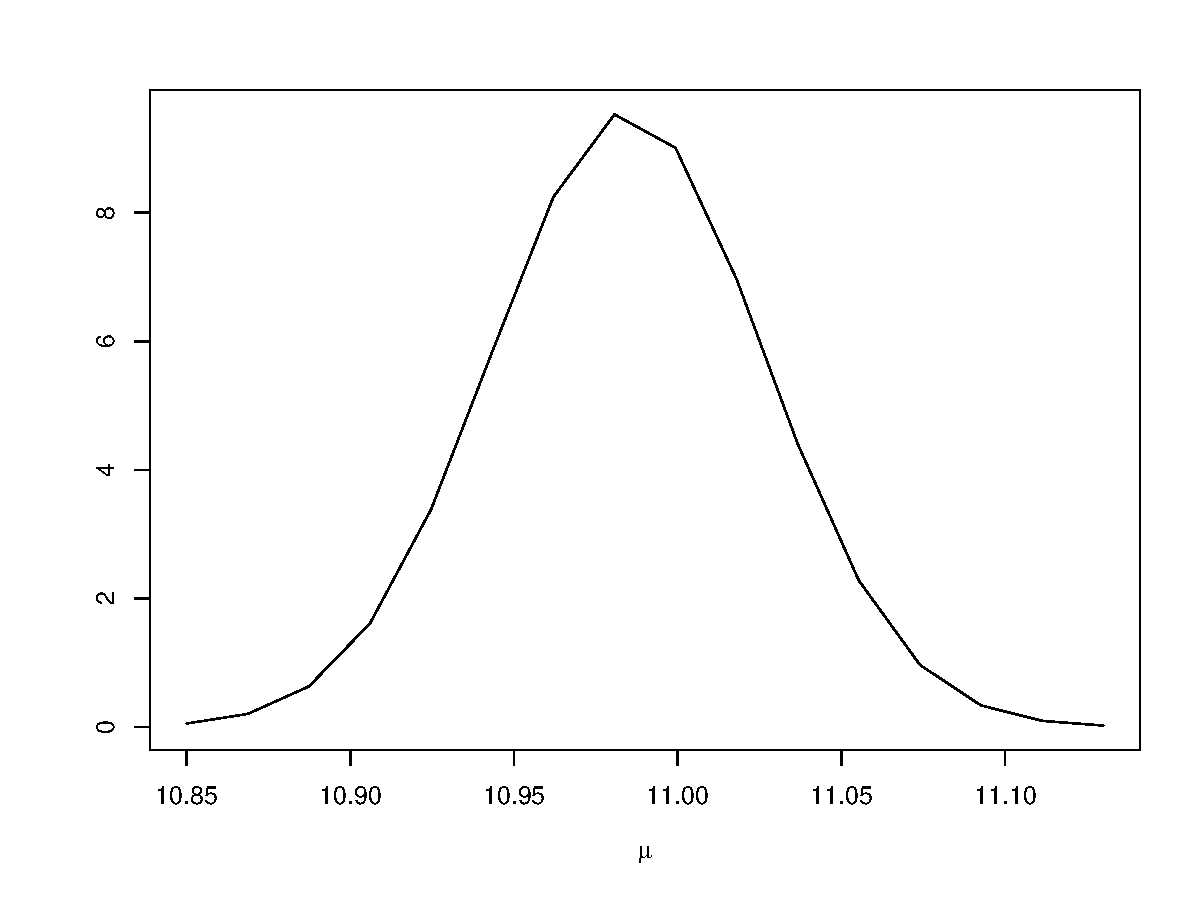
\includegraphics[scale=0.4]{figuras/dpm_mu_qr_15.pdf}}}%
	\qquad
	\subfloat[Densidade \textit{a posteriori} de $\sigma^2$]{{
			\label{fig:dpm_s2_qr_15}
			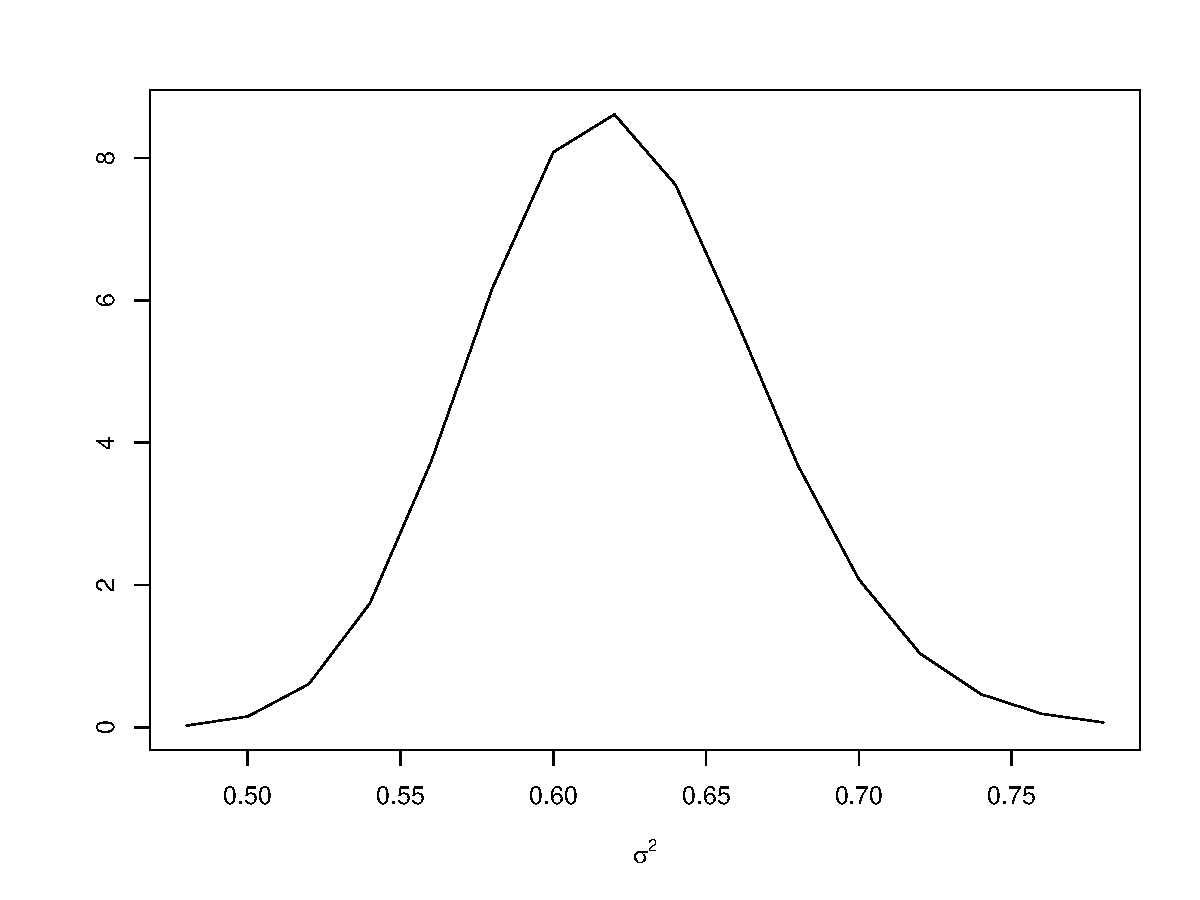
\includegraphics[scale=0.4]{figuras/dpm_s2_qr_15.pdf}}}%
	\subfloat[Densidade \textit{a posteriori} de $\nu$]{{
			\label{fig:dpm_nu_qr_15}
			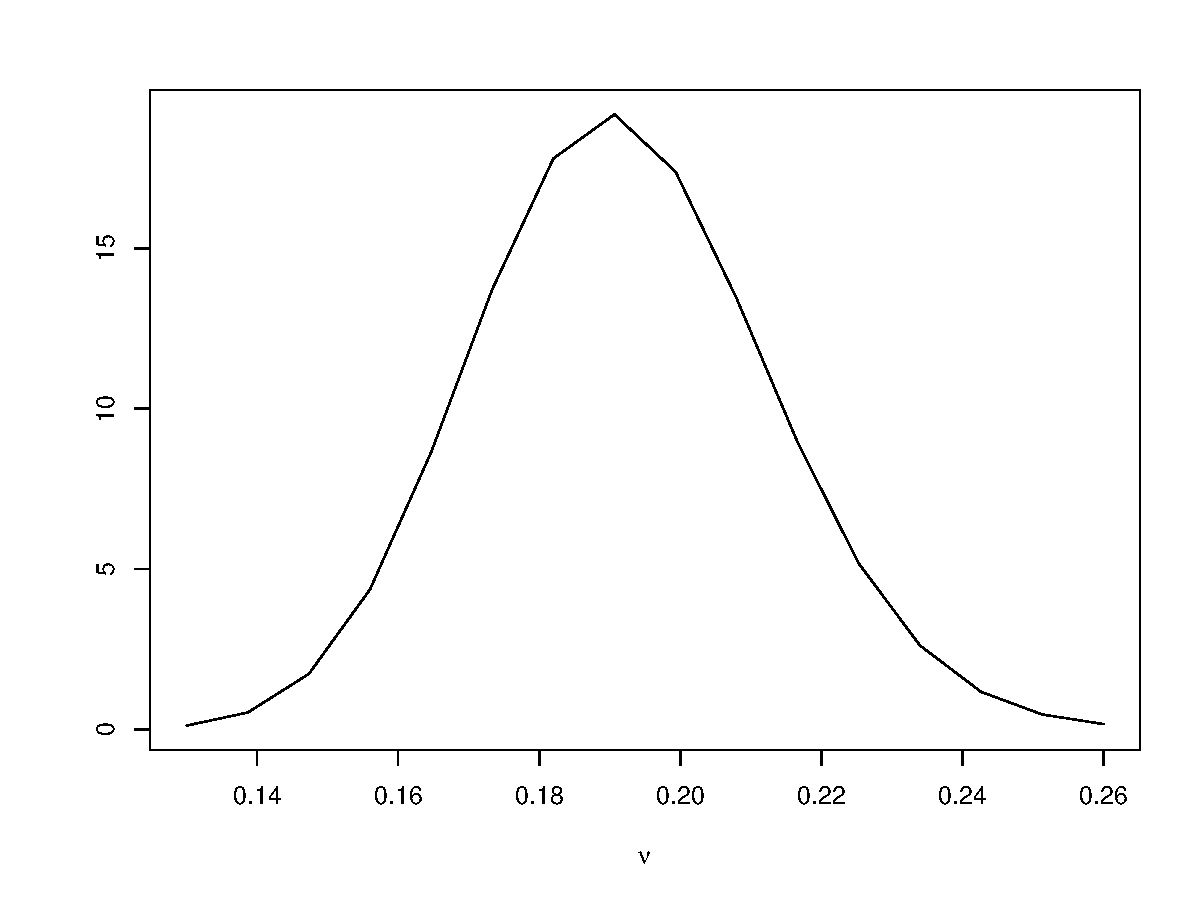
\includegraphics[scale=0.4]{figuras/dpm_nu_qr_15.pdf}}}%
	\caption{Densidades \textit{a posteriori} marginais pela quadratura de Riemann com $L = 15$}%
\end{figure}

\begin{figure}[t]%
	\centering
	\subfloat[Densidade \textit{a posteriori} de $\mu$]{{
			\label{fig:dpm_mu_qr_50}
			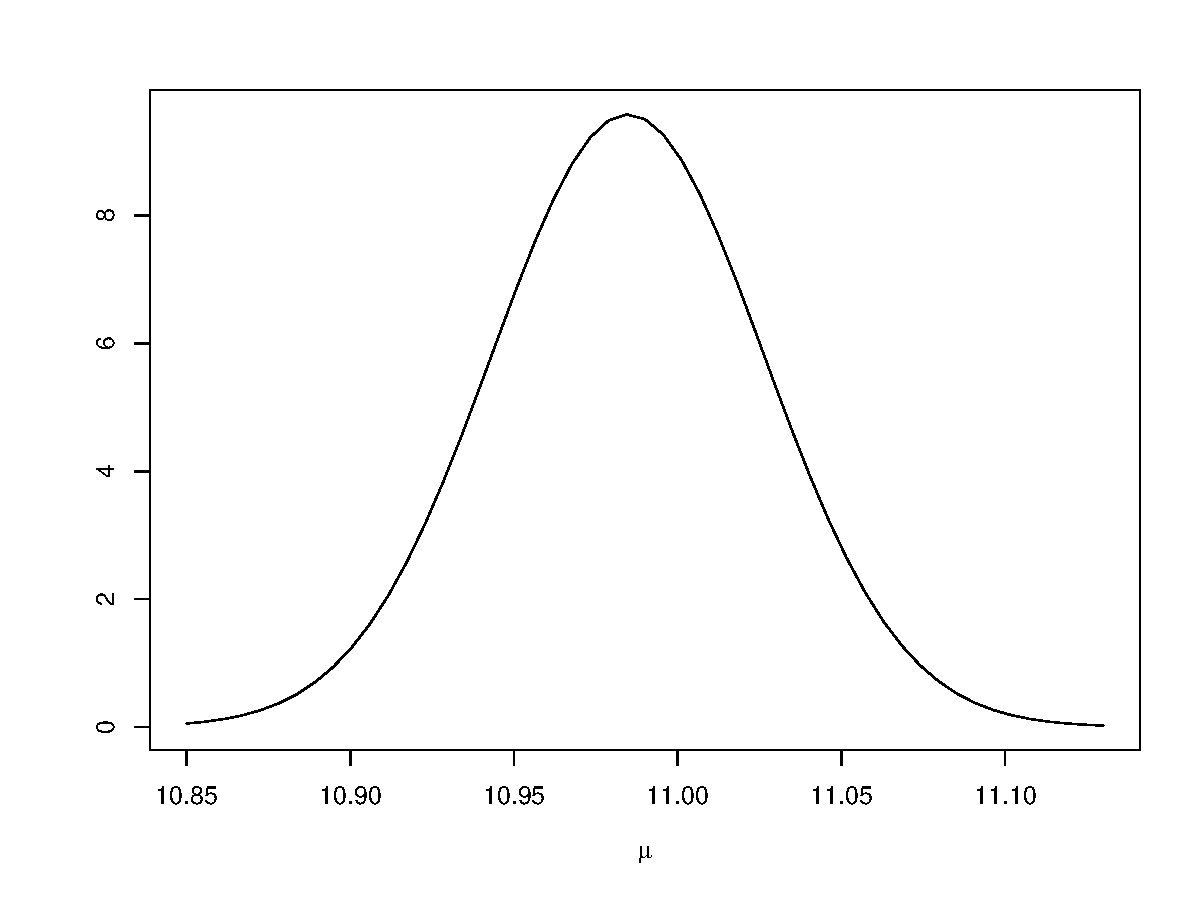
\includegraphics[scale=0.4]{figuras/dpm_mu_qr_50.pdf}}}%
	\qquad
	\subfloat[Densidade \textit{a posteriori} de $\sigma^2$]{{
			\label{fig:dpm_s2_qr_50}
			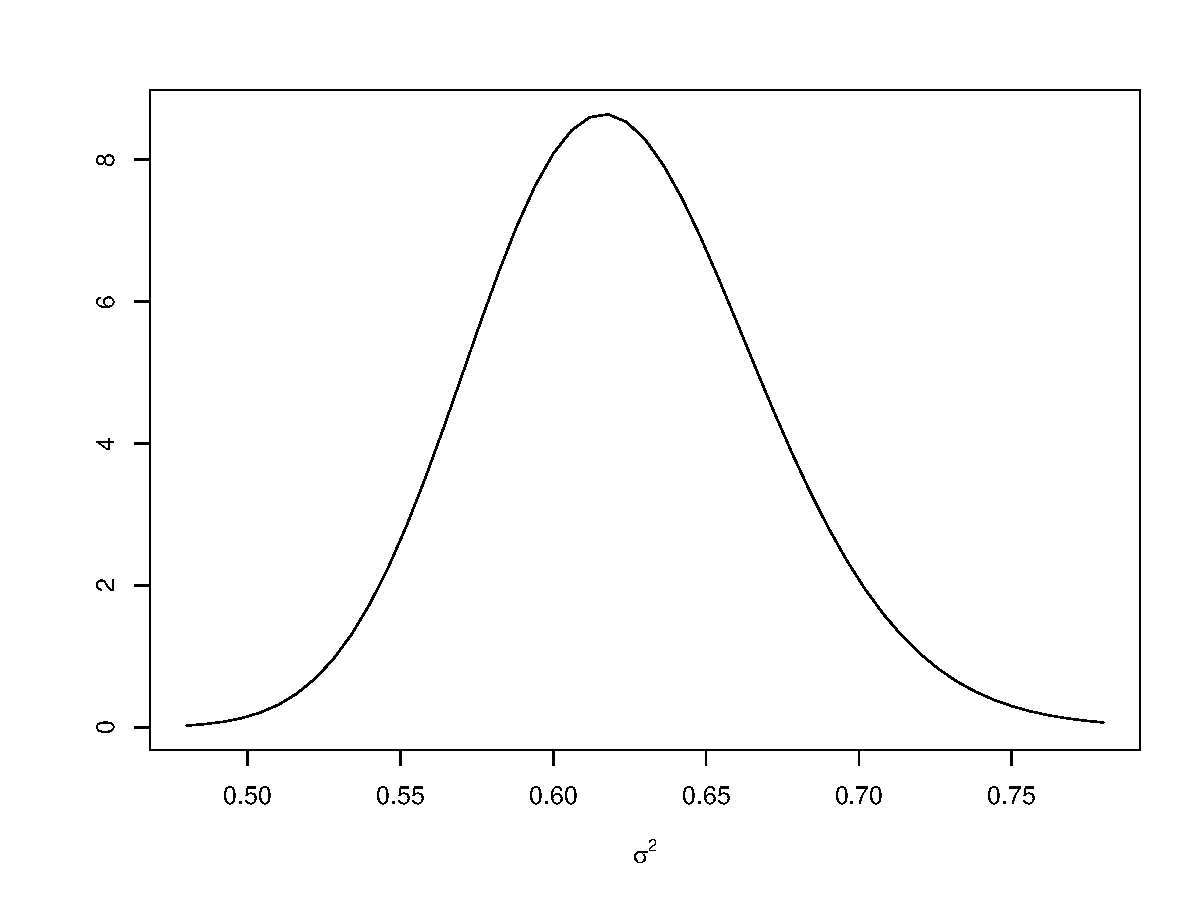
\includegraphics[scale=0.4]{figuras/dpm_s2_qr_50.pdf}}}%
	\subfloat[Densidade \textit{a posteriori} de $\nu$]{{
			\label{fig:dpm_nu_qr_50}
			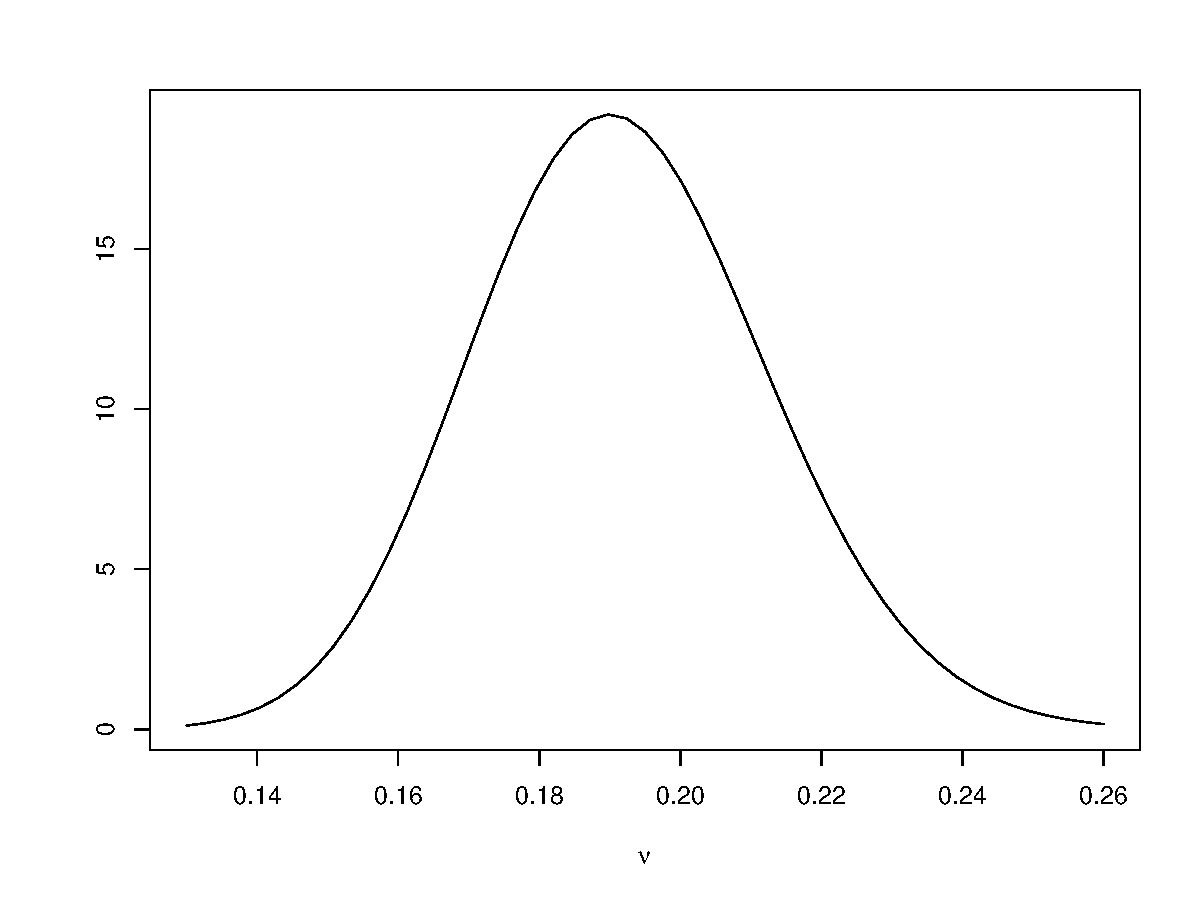
\includegraphics[scale=0.4]{figuras/dpm_nu_qr_50.pdf}}}%
	\caption{Densidades \textit{a posteriori} marginais pela quadratura de Riemann com $L = 50$}%
\end{figure}

\begin{figure}[t]%
	\centering
	\subfloat[Densidade \textit{a posteriori} de $\mu$]{{
			\label{fig:dpm_mu_qr_100}
			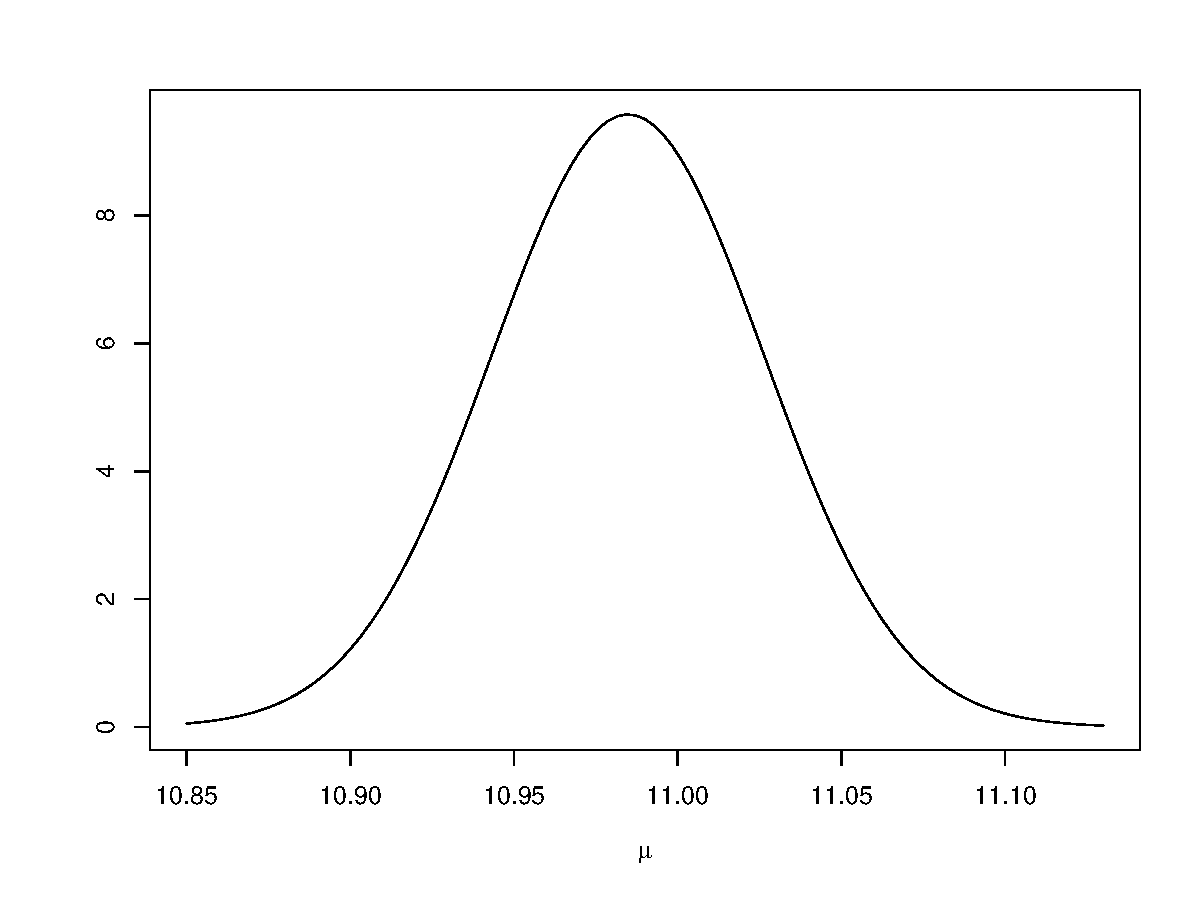
\includegraphics[scale=0.4]{figuras/dpm_mu_qr_100.pdf}}}%
	\qquad
	\subfloat[Densidade \textit{a posteriori} de $\sigma^2$]{{
			\label{fig:dpm_s2_qr_100}
			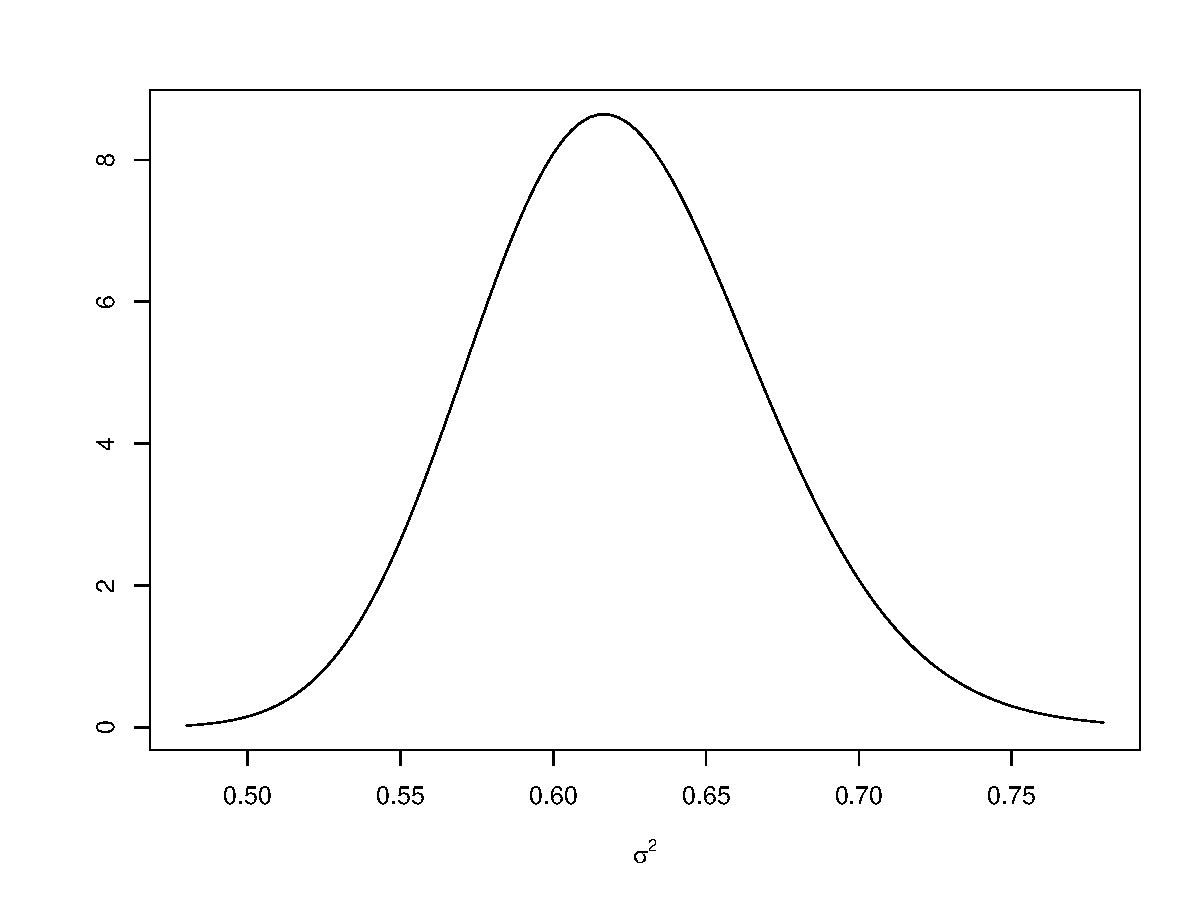
\includegraphics[scale=0.4]{figuras/dpm_s2_qr_100.pdf}}}%
	\subfloat[Densidade \textit{a posteriori} de $\nu$]{{
			\label{fig:dpm_nu_qr_100}
			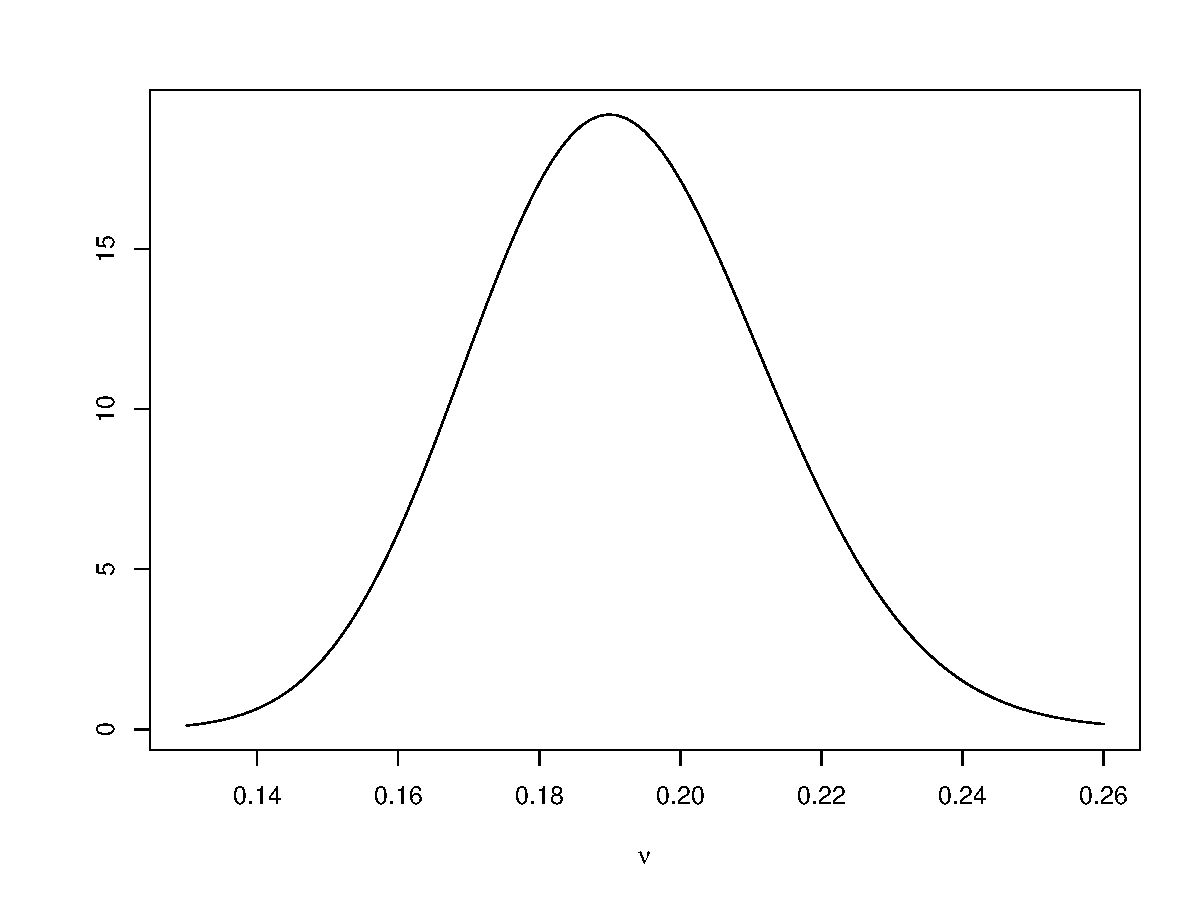
\includegraphics[scale=0.4]{figuras/dpm_nu_qr_100.pdf}}}%
	\caption{Densidades \textit{a posteriori} marginais pela quadratura de Riemann com $L = 100$}%
\end{figure}

Para $L=15$, a aproximação não é muito suave, mas começa a indicar como cada parâmetro se comporta com relação à locação e à dispersão de sua densidade \textit{a posteriori} marginal. Entretanto, ainda não é possível dizer como é o comportamento com relação à simetria.

Para $L=50$, a aproximação é bem suave. Além do comportamento com relação à locação e à dispersão, é possível dizer também como é o comportamento com relação à simetria da densidade \textit{a posteriori} marginal de cada parâmetro. Aparentemente, as densidades para $\sigma^2$ e $\nu$ são fracamente assimétricas à direita.

Para $L=100$, os gráficos confirma a tendência apresentada pelos dois cenários anteriores, mas com uma suavização ainda melhor. Porém, computacionalmente a integração numérica é bem mais demorada, uma vez que o número de pontos para cálculo das densidades \textit{a posteriori} marginais cresce a um fator de ordem $\mathcal{O}(L^3)$.

Obtidas as densidades \textit{a posteriori} marginais, é possível ainda estimar pela quadratura de Riemann os momentos \textit{a posteriori} de ordem $m$ para cada parâmetro e com os mesmos aproximar as estatísticas de média, variância, assimetria e curtose. Sem perda de generalidade, suponha que se deseja obter as estatísticas \textit{a posteriori} para $\alpha_1$. A aproximação pela quadratura de Riemann para um momento $m$ é dada por
\begin{align}
\mathbb{E}(\alpha_1^m | \bm{y}) &= \iint \alpha_1^m p(\alpha_1, \alpha_2, \alpha_3 | \bm{y}) d\alpha_1 d\alpha_2 d\alpha_3 \approx \sum_{i=1}^{L} \sum_{j=1}^{L} \sum_{k=1}^{L} r_i^m p(r_i, s_j, t_k | \bm{y}) \Delta_i \Delta_j \Delta_k \nonumber \\
&= \sum_{i=1}^{L} r_i^m \Delta_i \left[\sum_{j=1}^{L} \sum_{k=1}^{L} p(r_i, s_j, t_k | \bm{y}) \Delta_j \Delta_k\right] \nonumber \\
&= \sum_{i=1}^{L} r_i^m \Delta_i p(r_i | \bm{y}). \label{eq:mom_qr}
\end{align}

Como todas as estatísticas de interesse são funções dos quatro primeiros momentos, basta substituir $m = \{1, 2, 3, 4\}$ em \eqref{eq:mom_qr} para obter as respectivas aproximações. Na Tabela \ref{tab1}, são apresentados os valores aproximados para tais estatísticas em cada um dos três cenários.

\begin{table}[htb]
	\caption{Estatísticas \textit{a posteriori} para $(\mu, \sigma^2, \nu)$ pela quadratura de Riemann}
	\label{tab1}
	\centering
	\begin{tabular}{cccccc}
		\toprule
		Cenário & Parâmetro & Média & Variância & Assimetria & Curtose \\
		\midrule
		$L = 15$ & $\mu$      & 10.9847 & 0.0017 & 0.0022 & 2.9603 \\
		& $\sigma^2$ &  0.6222 & 0.0022 & 0.2230 & 2.9984 \\
		& $\nu$      &  0.1918 & 0.0004 & 0.1572 & 2.9348 \\
		\midrule
		$L = 50$ & $\mu$      & 10.9848 & 0.0017 & 0.0056 & 2.9346 \\
		& $\sigma^2$ &  0.6222 & 0.0021 & 0.2149 & 2.9625 \\
		& $\nu$      &  0.1918 & 0.0004 & 0.1523 & 2.8995 \\
		\midrule
		$L = 100$ & $\mu$      & 10.9848 & 0.0017 & 0.0064 & 2.9284 \\
		& $\sigma^2$ &  0.6222 & 0.0021 & 0.2131 & 2.9542 \\
		& $\nu$      &  0.1918 & 0.0004 & 0.1512 & 2.8913 \\
		\bottomrule
	\end{tabular}
\end{table}

Pela Tabela \ref{tab1}, pode-se concluir que tanto a média quanto a variância \textit{a posteriori} praticamente não variaram nos três cenários, independente do parâmetro considerado. Isto quer dizer que poucos subintervalos são necessários para se obter uma boa aproximação destas duas estatísticas. Por outro lado, o mesmo não pode ser dito para a assimetria e a curtose \textit{a posteriori}, para as quais há mudanças na terceira ou mesmo na segunda casa decimal, inclusive quando se passa de $L = 50$ para $L = 100$ subintervalos. Isto se explica pelo fato de que tanto a assimetria quanto a curtose são funções que dependem de vários momentos, até a terceira e quarta ordem respectivamente. Portanto, há maior dificuldade em aproximá-las. Apesar deste fato, para o problema considerado se pode dizer que houve uma estabilidade nas aproximações destas duas últimas estatísticas na medida em que a quantidade de subintervalos crescia.

Com relação aos valores em si, as médias \textit{a posteriori} para os 3 parâmetros ficaram bem próximas, mas não necessariamente iguais, aos respectivos valores do modelo para a distribuição amostral, mesmo para uma amostra muito grande ($n = 500$). É interessante notar que isso ocorre mesmo para o parâmetro $\nu$, cuja distribuição \textit{a priori} é não-informativa no sentido de Bayes-Laplace. Apesar disto, sua distribuição \textit{a posteriori} é influenciada pelas informações de $\mu$ e $\sigma^2$ contidas tanto nas distribuições \textit{a priori} correspondentes quanto na função de verossimilhança. Essa diferença já era esperada, uma vez que a aproximação é feita para a distribuição \textit{a posteriori} e não para a distribuição amostral.

Para as variâncias \textit{a posteriori}, todas elas foram bem pequenas, em especial para $\nu$. Isto se deve ao fato de que a amostra inicial dos dados era grande, portanto se poderia esperar uma redução na dispersão de cada parâmetro quando sua informação é atualizada com a distribuição amostral, por menos informativa que fosse a distribuição \textit{a priori} (como no caso de $\nu$). Com relação à assimetria \textit{a posteriori}, esta foi praticamente nula para $\mu$ e positiva, mas fraca, para $\sigma^2$ e $\nu$ (um pouco mais forte para a primeira). Por fim, as aproximações para a curtose \textit{a posteriori} foram todas bem próximas de 3, o valor encontrado para uma distribuição normal, com o parâmetro $\sigma^2$ mais próximo desse valor e $\nu$ o mais afastado.